%%%%%%%%%%%%%%%%%%%%%%%%%%%%%%%%%%%%%%%%%%%%%%%%%%%%%%%%%%%%%%%%%%%%%%%%%%%%%%%%
%2345678901234567890123456789012345678901234567890123456789012345678901234567890
%        1         2         3         4         5         6         7         8

\documentclass[letterpaper, 10 pt, conference]{ieeeconf}  % Comment this line out if you need a4paper

%\documentclass[a4paper, 10pt, conference]{ieeeconf}      % Use this line for a4 paper

\IEEEoverridecommandlockouts                              % This command is only needed if 
                                                          % you want to use the \thanks command

\overrideIEEEmargins                                      % Needed to meet printer requirements.

% See the \addtolength command later in the file to balance the column lengths
% on the last page of the document

% The following packages can be found on http:\\www.ctan.org
\usepackage{graphics} % for pdf, bitmapped graphics files
\usepackage{epsfig} % for postscript graphics files
\usepackage{mathptmx} % assumes new font selection scheme installed
\usepackage{times} % assumes new font selection scheme installed
\usepackage{amsmath} % assumes amsmath package installed
\usepackage{amssymb}  % assumes amsmath package installed
\usepackage{subcaption}  % assumes amsmath package installed
\usepackage{graphicx}
\usepackage{algorithm}
\usepackage{algorithmic}
\usepackage{caption}

\newcommand{\tabref}[1]{Table~\ref{tab:#1}}
\newcommand{\tablab}[1]{\label{tab:#1}}
\newtheorem{lemma}{Lemma}
\newtheorem{theorem}{Theorem}
\newcommand{\tab}[1]{\hspace{.02\textwidth}\rlap{#1}}
\newcommand{\alglab}[1]{\label{alg:#1}}
\newcommand{\algref}[1]{Algorithm~\ref{alg:#1}}
\newcommand{\eqnref}[1]{Equation~\ref{eqn:#1}}
\newcommand{\figref}[1]{Figure~\ref{fig:#1}}
\newcommand{\figlab}[1]{\label{fig:#1}}
\newcommand{\eqnlab}[1]{\label{eqn:#1}}
\newcommand{\eg}{G^{E}}
\newcommand{\heg}{h^{E}}
\newcommand{\eeg}{\varepsilon^{E}}
\DeclareMathOperator*{\argmin}{arg\,min}

\title{\LARGE \bf
Lazy Validation of Experience Graphs
}
	
\author{
\authorblockN{Victor Hwang}
\authorblockA{vchwang@andrew.cmu.edu\\
Carnegie Mellon University}
\and
\authorblockN{Mike Phillips}
\authorblockA{mlphilli@andrew.cmu.edu\\
Carnegie Mellon University}
\and
\authorblockN{Siddhartha Srinivasa}
\authorblockA{siddh@cs.cmu.edu\\
Carnegie Mellon University}
\and
\authorblockN{Maxim Likhachev}
\authorblockA{maxim@cs.cmu.edu\\
Carnegie Mellon University}
}

%\author{\authorblockN{Victor Hwang}, Mike Phillips, Siddhartha Srinivasa, Maxim Likhachev% <-this % stops a space
%\thanks{*This work was not supported by any organization}% <-this % stops a space
%\thanks{$^{1}$Albert Author is with Faculty of Electrical Engineering, Mathematics and Computer Science,
%        University of Twente, 7500 AE Enschede, The Netherlands
%        {\tt\small albert.author@papercept.net}}%
%\thanks{$^{2}$Bernard D. Researcheris with the Department of Electrical Engineering, Wright State University,
%        Dayton, OH 45435, USA
%        {\tt\small b.d.researcher@ieee.org}}%
%}


\begin{document}



\maketitle
\thispagestyle{empty}
\pagestyle{empty}


%%%%%%%%%%%%%%%%%%%%%%%%%%%%%%%%%%%%%%%%%%%%%%%%%%%%%%%%%%%%%%%%%%%%%%%%%%%%%%%%
\begin{abstract}

Many robot applications involve lifelong planning in relatively static
environments e.g. assembling objects or sorting mail in an office building.  In
these types of scenarios, the robot performs many tasks over a long period of
time. Thus, the time required for computing a motion plan becomes a significant
concern, prompting the need for a fast and efficient motion planner.  Since
these environments remain similar in between planning requests, planning from
scratch is wasteful. We propose using Experience Graphs (E-Graphs) to accelerate
the planning process by reusing parts of previously computed paths to solve new
motion planning queries more efficiently.  This work describes a method to
improve planning times with E-Graphs given changes in the environment by lazily
evaluating the validity of past experiences during the planning process. We show
the improvements with our method in a single-arm manipulation domain with
simulations on the PR2 robot.

\end{abstract}


%%%%%%%%%%%%%%%%%%%%%%%%%%%%%%%%%%%%%%%%%%%%%%%%%%%%%%%%%%%%%%%%%%%%%%%%%%%%%%%%
\section{Introduction}
In situations where a robot is doing lifelong planning, the efficiency of a
motion planner becomes very important. However, in tasks such as assembling
objects or performing sorting and pick-and-place tasks, motion planners still
suffer from poor planning times depending on the complexity of the environment.
In a robot manipulation environment, it is simple to find standard scenarios
where planning takes a non-trivial amount of time, despite the fact that these
environments are relatively structured.

In this work, we leverage learning from prior experiences to tackle difficult
planning scenarios where a robot's movement in a structured environment is
encumbered by unpredictable clutter. \figref{mailroom} shows a mailroom environment,
where the general task of sorting mail is a structured one. However, this
environment typically has clutter appearing inside cubby holes or on shelves.
By learning from experiences, we expect a mail-sorting robot to accumulate
enough experience over time so that planning to constrained spaces (cubbyholes,
boxes, etc) becomes very fast. At the same time, we expect this framework to be
robust against the fact that portions of its prior experiences are constantly
becoming invalid due to clutter.

Our work modifies an existing Experience Graph planner \cite{PhillipsRSS:2012} to provide
fast planning times in this kind of challenging environment. The Experience
Graphs (E-Graphs) framework acts as a collection of previously planned
paths and augments A*-like searches to guide a search to reuse these past
experiences. This results in faster planning times while maintaining
completeness guarantees and a bound on the sub-optimality of the solution with
respect to the optimal path.

While \cite{PhillipsRSS:2012} provides an efficient planning framework for a completely
static environment with a large number of prior experiences, planning times
suffer once the possibility of unpredictable clutter is introduced. The
E-Graph planner is only able to plan with a completely valid set of experiences;
even a negligible change in the environment forces the planner to validate its
entire set of experiences to ensure a valid plan. Considering the robot may be
working tirelessly for long periods of time, the E-Graph can grow substantially
and introduce more and more overhead into every single planning request.  

\begin{figure}
    \centering
    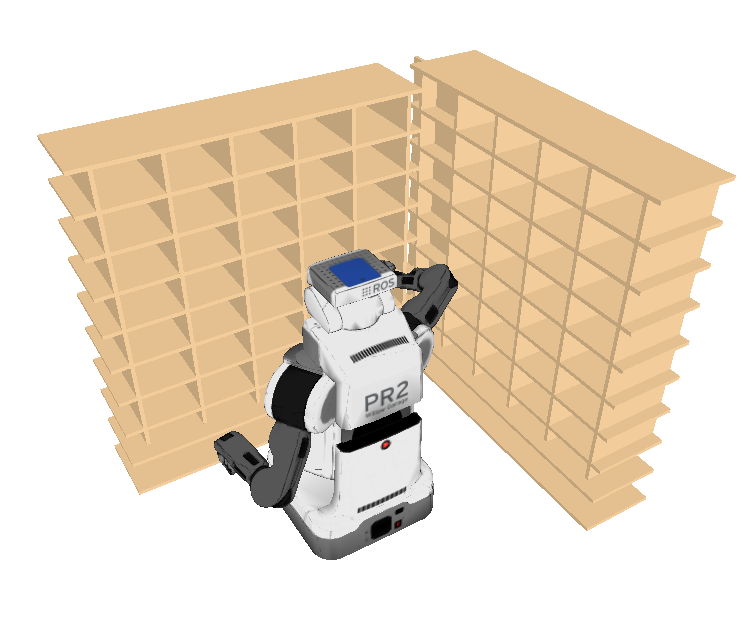
\includegraphics[scale=.3]{basic_env.png}
    \caption{PR2 in a simulated mailroom environment.}
    \figlab{mailroom}
\end{figure}

In this paper, we address one facet of the problem that affects any data-driven
algorithm: \emph{does it scale}? We show efficient experience validation by
introducing a lazy method that only validates prior experiences that the planner
deems potentially relevant to the planning task. This method leads to
performance improvements in changing, cluttered environments. Specifically, we
show speedups using a simulated environment where the PR2 conducts single arm,
7D manipulation tasks in a constrained mailroom environment.

\section{Related Work}
Motion planning has seen considerable interest recently. Most of the
approaches were initially focused on treating each new motion planning request as
a fresh request for planning. There was little, if any, reuse of information
from experience gained while carrying out a series of motion plans. However,
recent work has seen more reuse of previous information. In \cite{Lien:2005},
Lien et.  al. constructed roadmaps for obstacles, stored them in a database and
reused them during motion planning while Bruce et. al.~\cite{Bruce:2002} biased
an RRT search towards waypoints remembered from previous motion planning
attempts. Related work can also be found in~\cite{Zucker:2007,Ferguson:2006}.

Other approaches to exploiting experience have included the use of trajectory
libraries. These libraries were used to adapt policies for control of
underactuated systems and high-dimensional systems in~\cite{Stolle:2006}. In~
\cite{Atkeson:2003}, entirely new trajectories were generated by combining
nearby trajectories. A different application of such techniques can also be
found in~\cite{Liu:2009} while transfer of policies across tasks was presented
in~\cite{Stolle:2007}. The reuse of environment information, coupled with
information about previous motion plans, was presented in~\cite{Jetchev:2010};
machine learning methods were coupled with paths stored in a database to
generate new motion plans based on the environment and types of obstacles. Jiang
et. al.~\cite{Jiang:2007} present an approach to use a database of older
motion plans to draw a bi-directional RRT search towards a path stored in the
database that is most similar to the new motion plan request.  Recent
work~\cite{Berenson:2012} attempts to repair previous plans from a database
using randomized planners. As mentioned in~\cite{PhillipsRSS:2012}, the use of a
database of motion plans is also core to Experience Graphs. 

Search-based planning with Experience Graphs offers several advantages over
these approaches. Experience Graphs attempt to use all information from
previous experiences instead of attempting to find the nearest or closest motion
plan from a database. They are thus capable of reusing many parts of the previous
experiences when possible. This method provides guarantees on completeness and
solution quality, which the other methods lack.
It also builds the graph using paths from prior tasks in contrast
to approaches like Probabilistic Roadmaps ~\cite{Kavraki:1996} which rely on
sampling the whole space. At the same time, there are parallels between the Lazy
Probabilistic Roadmap \cite{bohlin2000path} and the work we present in that both
methods only do expensive validation once a plan has been generated.

\section{Experience Graphs}

This section provides a brief overview of the E-Graphs framework. For a more
in-depth analysis, see ~\cite{PhillipsRSS:2012}.

E-Graphs augment A* search to reduce search computation by reusing relevant
pieces of prior experience. It is composed of two aspects - the Experience Graph
that maintains all the prior experience, and a heuristic that drives a weighted
A* search towards these prior experiences during the planning process.

The Experience Graph $G^E$ maintains a collection of previously planned paths as
a set of edges $E^E$ and vertices $V^E$. While weighted A* still
searches the original graph $G$, a new heuristic function $h^E(s)$ is introduced
that encourages the search to explore $G^E$ rather than $G$:

\begin{equation}
\heg(s_0) = \underset{\pi}{min} \sum\limits_{i=0}^{N-1} min \lbrace \eeg h^G(s_i,s_{i+1}), c^{E}(s_i,s_{i+1}) \rbrace 
\eqnlab{heur}
\end{equation}

In \eqnref{heur}, $h^E(s)$ is defined as computing the cost of the shortest path $\pi$
where $\pi$ is a path $\langle s_0 \dotsc s_{N-1} \rangle$ and
$s_{N-1}=s_{goal}$.  This path is constructed using two kinds of edges. The
first edge cost, $\epsilon^Eh^G(s_i, s_{i+1})$, represents the original search
heuristic $h^G(s,s')$ and describes the underestimating cost between states
$s$ and $s'$ for all states in $G$. The second term represents the edge cost
$c^E(s, s')$ between states on $G^E$. The scalar $\epsilon^E$ is a parameter to
inflate the cost of the first term to favor the second. This effectively
forces the minimum path to avoid using edges not on the E-Graph and
instead, favor using edges from previous experiences.

\begin{figure}
\centering
%\figlab{egraph}\includegraphics[width=0.4\columnwidth]{plain_old_egraph.ps}
\figlab{heur_1}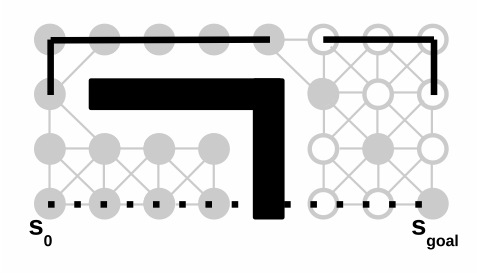
\includegraphics[width=0.8\columnwidth]{eps1.png}
\figlab{heur_inf}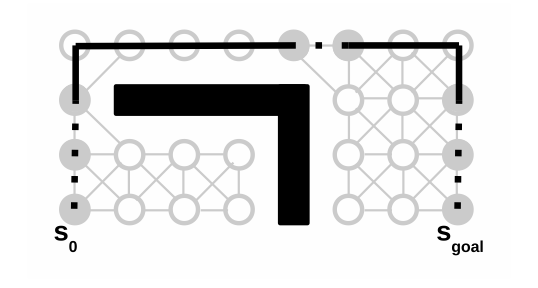
\includegraphics[width=0.9\columnwidth]{eps_inf.png}
\caption{The above two images show the differences between heuristics when varying
    $\eeg$. When $\eeg$ is close to one, the heuristic effectively becomes $h^G$
    (in this example, Euclidean distance), as seen in the top image. The dashed
    line indicates that it is a heuristic edge. As $\eeg$ increases, the
    heuristic guides along previous experiences, as shown by the solid lines in
    the bottom figure.
}
\vspace{-4mm}
\figlab{heur}
\end{figure}

The qualitative effect of $\epsilon^E$ can be seen in \figref{heur}.  This image
shows the search from $s_0$ to $s_{goal}$ and the required state expansions to
find the solution. In both images, the grey circles represent states expanded
during the search and the solid black line represents a E-Graph edges of a prior
experience. We use Euclidean distance as the original heuristic $h^G$, which is
represented as the dashed line. When the $\epsilon^E$ is close to one,
$h^\epsilon$ draws the search directly towards the goal with a heuristic edge
(dashed line) and avoids using any E-Graph edge. However, this heuristic
guidance isn't particularly helpful, since the search is led straight into an
obstacle (black rectangles). We see that many states end up being expanded
(shown in gray). As
$\epsilon^E$ increases (bottom image), $h^\epsilon$ instead guides the search
towards the prior experience (black lines), which effectively dodges the
obstacle and completes the search with fewer states expanded.

In \cite{PhillipsRSS:2012}, it was shown that this heuristic is $\epsilon^E$
consistent and therefore it is guaranteed that the solution cost will be no
worse than $\epsilon^E$ times the cost of the optimal solution when finding a
path using A* search. Because weighted A* inflates $h^E$ by $\epsilon$, the cost
of the solution is bounded by $\epsilon \cdot \epsilon^E$ times the optimal
solution cost.

\subsection{Experience Graph Shortcuts}
One important element to the E-Graph algorithm is the use of shortcuts. E-Graph
shortcuts are a mechanism for further reducing the number of expansions by
introducing a new type of successor $s_{shortcut}$ to the search.  
Given a connected component $C$ where $C \subseteq
V^E$ 
\begin{equation}
s_{shortcut} = \argmin_{s \in C} h^E(s)
\eqnlab{shortcut}
\end{equation}

When expanding any state $s \in C$, 
$s_{shortcut}$ becomes an additional valid successor of $s$, allowing the search
to avoid expanding intermediate states in $C$.

\begin{figure}
    \centering
    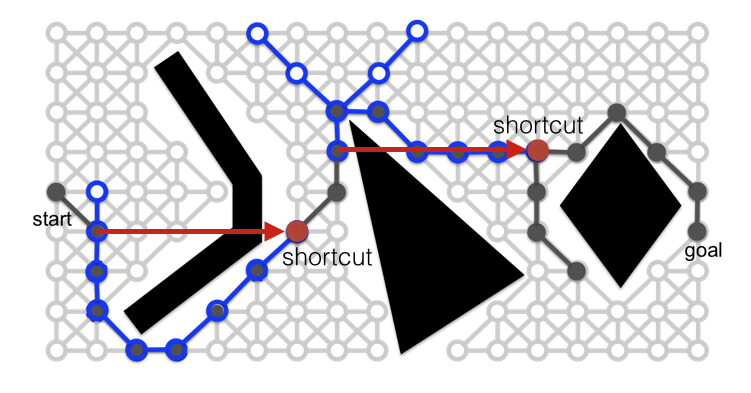
\includegraphics[width=1\columnwidth]{shortcut.png}
    \caption{An example of shortcut successors (arrows) being used to avoid
    expanding unnecessary states on an E-Graph component.}
    \figlab{myshortcut}
\end{figure}

In \figref{myshortcut}, we see two components that are not directly connected to
the goal. For each component, we compute a shortcut state as per
\eqnref{shortcut}, generating the two labeled nodes. The arrows show an example
of expanding one node on the component, which has the shortcut node as a
successor. This leads to the planner avoiding expanding states along a
particular E-Graph component by jumping right to the end. 

The utility of this successor can be seen more clearly when similar start/goal
pairs are repeatedly solved by the planner (assuming a valid E-Graph). The first
instance of planning for a given pair will result in many expansions. However,
subsequent expansions will only require expanding a few additional node besides
the start, and will immediately end up at the goal state, regardless of how many
E-Graph edges lie in between the start and goal.

\section{Lazy Validation of E-Graphs}

This section describes the lazy validation of E-Graphs. The algorithm is built
on top of the original E-Graph planner described in \cite{PhillipsRSS:2012}; it
uses the same heuristic computation to focus the search towards prior
experiences.  However, rather than maintaining E-Graph feasibility and validity as
an invariant, we loosely assume that the E-Graph is valid until the E-Graph planner
returns a complete solution.  Only then do we validate the vertices and edges in
the solution path that lie on the E-Graph.


\begin{algorithm}{lazyPlan}($s_{start}, s_{goal}, G^E$)
    \begin{algorithmic}[1]
        {\footnotesize 
    \STATE while not valid $\pi$ do:
    \STATE \tab{$initializeEGraph(s_{goal})$}
    \STATE \tab{$\pi = computePath(s_{start}, s_{goal})$}
    \STATE \tab{if $\pi$ is not valid:}
    \STATE \tab{\tab{$G^E = G^E \cup \pi$}}
    \STATE \tab{\tab{$(V_{invalid}, E_{invalid}) = returnInvalidElements(\pi)$}}
    \STATE \tab{\tab{$G^E = G^E \setminus (V_{invalid},
    E_{invalid})$}}
\STATE $return \, \pi$
}
\end{algorithmic}
\caption{}
\alglab{plan}
\end{algorithm}

\begin{algorithm}{initializeEGraph}($s_{goal}$)
    \begin{algorithmic}[1]


\STATE $precomputeShortcut$
\STATE compute heuristic according to \eqnref{heur}
\end{algorithmic}
\caption{}
\alglab{initializeEGraph}
\end{algorithm}


\algref{plan} shows a high level overview of the logic.  Given a pre-built
E-Graph $G^E$, we run the standard procedure for E-Graph planning: initializing
relevant E-Graph mechanisms (\algref{initializeEGraph}), which pre-computes the
shortcuts and the E-Graph heuristic. Once we compute a path $\pi$, we feed it
back into the E-Graph.  In $returnInvalidElements$, we validate elements of
$G^E$ related to  $\pi$ and return those that are invalid. In line 7, we
remove these from $G^E$, and rerun the planning cycle. Given that the E-Graph
contains a sufficient amount of experience and the environment has not change
dramatically, the number of total replans remains low.

The goal of $returnInvalidElements$ goes beyond discovering points on the
returned path that are invalid. Because the while loop continues to run until a
valid path is returned, it is advantageous to discover as many invalid edges and
vertices in $G^E$ as possible in a single run of $returnInvalidElements$,
especially those that are not explicitly part of $\pi$.  In the ideal case, one
could run a pre-computation to determine vertex connectivity in terms of the
validation procedure., i.e. return all $V_{invalid}$ given that a particular
vertex is invalid. However, this is likely computationally expensive, so faster
approximations can be used.

In our implementation of lazy E-Graphs for robot arm planning, we check that the
3D location of the end effector for $V_{invalid}^\epsilon$ is not an obstacle.
If it is, we look up all other $V^E$ that result in the same end effector
position, and invalidate those as well.

\begin{figure}[H]
    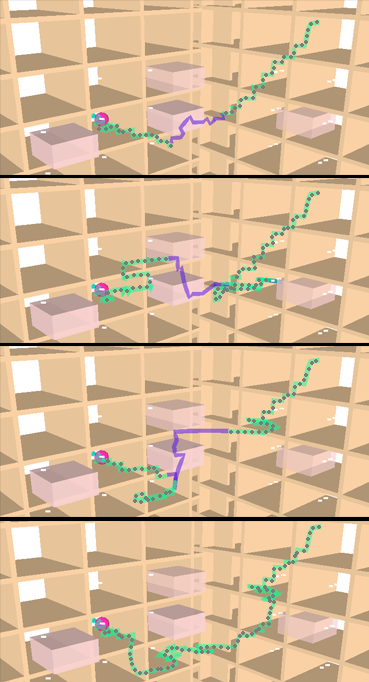
\includegraphics[width=1\columnwidth]{four_itrs.png} \caption{Four
        iterations of the lazy validation method. While the plans are
        7-dimensional, the pictures show their corresponding end-effector
        trajectories. The dark regions in the top three images show the invalid
        regions of the end effector path, while the dotted lines are the valid
    regions of the path. The last image shows a final (without shortcutting) path of
the end effector.  }
    \figlab{itrs}
\end{figure}

An example run of the lazy method can be seen in \figref{itrs}. Three
replans are required before a completely valid path is found in the fourth
image.

\subsection{Theoretical Properties}
While this replanning step can repeat many times, the framework still maintains
theoretical guarantees described in \cite{PhillipsRSS:2012}. Specifically, there
is an upper limit on the solution cost with respect to the optimal cost. 

\begin{theorem}
    \textit{For a finite graph $G$, and finite graph $G^E$, the planner
    terminates and finds a path in $G$ if one exists. }
\end{theorem}

\begin{theorem}
    \textit{For a finite graph $G$, and finite graph $G^E$, the planner
terminates and the solution returned is no worse than $\varepsilon \cdot \eeg$  times
the optimal solution cost in $G$.}
\end{theorem}

\section{Experimental Results}

We tested our approach in a simulated mailroom environment, where the PR2 robot
is sorting objects between cubby holes, as seen in \figref{mailroom}. We use an
existing benchmarking framework to run all experiments \cite{cohen2012generic}.
All the tasks involve manipulation with a single 7DOF arm of the PR2. The goals
are specified as the position and orientation of the end effector.

\begin{figure}[H]
    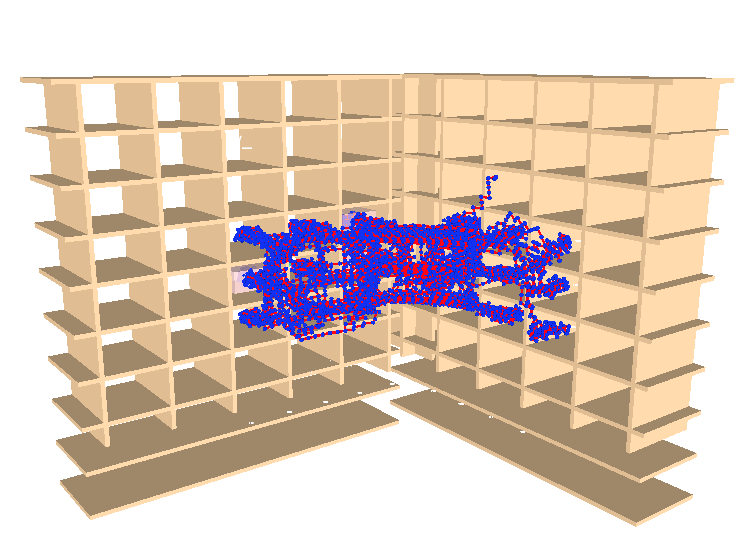
\includegraphics[width=1\columnwidth]{egraph.png}
    \caption{An E-Graph with 7000 vertices. Each vertex represents the end
        effector location of a state, and edges represent the 3D movement of the
    end effector.}
    \figlab{egraph}
\end{figure}

We first build up a usable E-Graph by running 200 trials of random start goal
pairs between the 18 cubby holes in the environment. These 200 trials are run
with a very low bound ($\varepsilon=1.5$) to ensure high quality experiences
between locations. This results in an E-Graph of near 7000 vertices.
\figref{egraph} shows a visualization of the E-Graph - each vertex represents
the 3D location of the end effector of a particular $V^G$ and the edges
represent end effector motions.

For testing, we run 50 trials where each trial introduces six randomly placed
obstacles inside the cubbies. We plan using three different E-Graph based
methods and the OMPL \cite{ompl} implementation of the RRT. We do not report
any results for Probabilistic Roadmaps or RRT* since they were
both unable to successfully plan in this scenario. For the E-Graph based
methods, we plan with a higher $\epsilon$ and $\epsilon^E$, allowing for more
reuse of experiences. All paths undergo shortcutting in a post-processing phase.
After each trial, the E-Graph is reloaded with the 200 trial training set. All
statistics are computed on trials where all the planners succeed.


We compare lazy validation with two other similar methods: full validation and
on-the-fly validation. In full validation, we validate every vertex and edge in
$G^E$ once a planning request has been received. This computation is factored
into the planning time.  The on-the-fly validation method incorporates the
validity check of E-Graph edges into the search itself - successors of a state
are thrown out if they utilize any invalid E-Graph edge. \algref{plan}, on the
other hand, returns a complete path before any E-Graph edges are invalidated.
In all algorithms, the validation of any E-Graph edge is equivalent to running a
full collision check of the robot arm against the environment.

\begin{table}[h]
    \begin{center}
        \begin{tabular}{| l | l | l | l | l | }
            \hline
            & Lazy & Full & On-the-fly & RRTConnect \\ \hline
            Median CC/request & 5280 & 54235 & 8304 & 191248 \\ \hline
            Average CC/request & 14222 & 54245 & 11574 & 221606\\ \hline
        \end{tabular}
    \end{center}
    \caption{Collision check count comparison between three E-Graph methods and
    RRTConnect. All E-Graph methods are initialized with an E-Graph of 7000
vertices.}
    \tablab{cccount}
\end{table}

\begin{table}[h]
    \begin{center}
        \begin{tabular}{| l | l | l | l | l | }
            \hline
            & Lazy & Full & On-the-fly & RRTConnect \\ \hline
            Fast CC & 1.45 & 1.24 & .97 & 8.99 \\ \hline
            Medium CC & 2.44 & 6.83 & 1.76 & 42.3\\ \hline
            Slow CC & 7.16 & 29.9 & 5.09 & 98.4 \\ \hline
            Success Rate& 76\% & 80\% & 73\% & 84\% \\ \hline
        \end{tabular}
    \end{center}
    \caption{Average planning time in seconds using different speeds of
    collision checkers. The "fast" collision checker takes $2.0\times10^{-5}$
sec/collision check. The ``medium" collision checker takes $1.1\times10^{-4}$
sec/collision check. The ``slow" collision checker takes $4.9\times10^{-4}$
sec/collision check. As a reference, the SBPL approximate collision checker is
the ``fast" checker. The FCL collision checker is slightly slower than our
``medium" collision checker at $2.4\times10^{-4}$ sec/collision check.
}
    \tablab{ptimes}
\end{table}

The first experimental result we present is statistics on the number of
collision checks that each planner issued. Because collision checking generally
takes up a large portion of planning times, this offers an
implementation-independent view of performance (compared to planning times, which
depend on the particular collision checking implementation).  \tabref{cccount}
shows both the median and average number of collision checks for all planning
methods. We see that the lazy and on-the-fly methods have lower average
collision checks overall.  We expect full validation to have a high average,
because it's directly proportional to the number of E-Graph vertices. RRTConnect
has a difficult time in this environment, with an order of magnitude
more collision checks due to the narrow passages from the cubbies.

In order to get a sense of planning times, one experiment was run to demonstrate
the planning times for different speeds of collision checkers.  We begin with
the SBPL collision checker, which operates very quickly because of its
sphere-based approximate model of the robot. However, in domains where a robot
is manipulating objects, an exact collision checking model may be required, such
as the Flexible Collision Library \cite{pan2012fcl}.  

\begin{figure}[ht]
    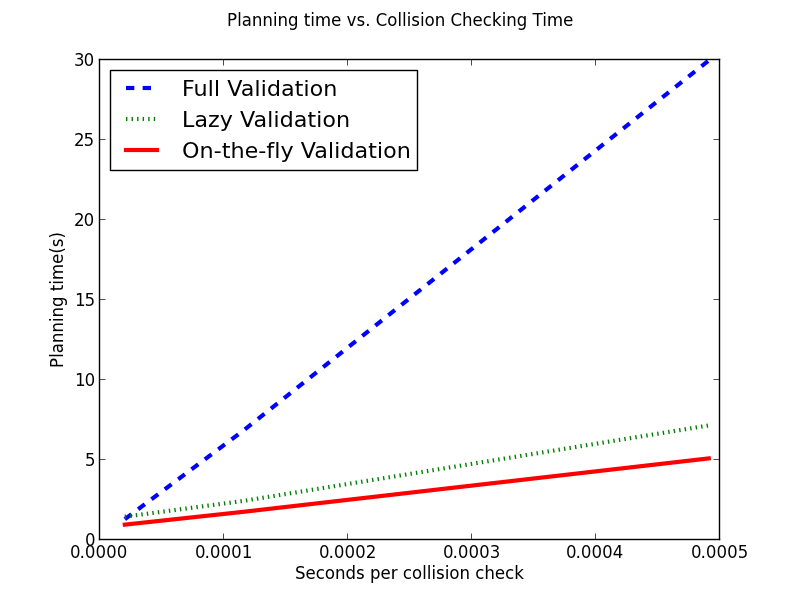
\includegraphics[width=1\columnwidth]{full_lazy_onthefly2.png}
    \caption{A comparison between the lazy validation and full validation method
    over different speeds of collision checking. These results were generated by
artificially slowing the SBPL collision checker performance to various speeds. }
    \figlab{cccompare}
\end{figure}

To get a sense of how the E-Graph methods scale with time required for a single
collision check, we artificially increase the amount of computation in the SBPL
collision checker \cite{cohen2013single} to various speeds and measure the required planning time.
\figref{cccompare} shows a plot of the planning times, and \tabref{ptimes} shows
the times for several speeds of the collision checker. Overall, we see the clear relationship that, as collision
checking time increases, full validation linearly increases in planning time,
while lazy validation and on-the-fly validation do not suffer.  As a reference,
FCL takes roughly $2.4\times10^{-4}$ seconds per collision check. Interpolating
on our results, FCL would spend about 12 seconds to plan for full validation,
while lazy validation still remains close to two seconds. 

We see that the on-the-fly is slightly faster in planning time than the lazy
method.  However, this is due to a fundamental difference that actually makes
the on-the-fly method inferior to the lazy method. The on-the-fly changes the
E-Graph during the search process, which results in the precomputed heuristic
becoming less and less informative. In fact, simple scenarios can be found where
on-the-fly will fail to plan due to a completely misdirected heuristic. 

\begin{figure}[ht]
    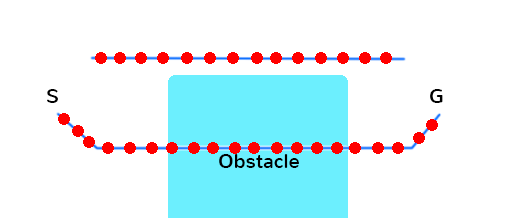
\includegraphics[width=1\columnwidth]{ontheflyprob7.png}
    \caption{A scenario where on-the-fly validation will fail due to a
    misinformed heuristic, whereas lazy validation will succeed. Before any
invalidation occurs, the heuristic guides the search along the bottom path. When
both methods discover that the experience passes through the obstacle, the
corresponding edges are invalidated. Lazy validation will recompute the
heuristic and guide the search towards the top segment of experience.
On-the-fly, however, will not recompute the heuristic, and get stuck trying to
bypass the obstacle.}
    \figlab{ontheflyprob}
\end{figure}

This is illustrated in \figref{ontheflyprob}. We begin with a two paths leading
to the goal. When we introduce an obstacle that obstructs one of the prior
experience, a segment of the experience is taken out. At this point, we hope
that the method will use the second path to the goal to quickly find a solution.
Because the lazy validation method reruns the heuristic computation every time
the heuristic is invalidated, the search will be lead to the second path. The
on-the-fly method's heuristic, however, becomes woefully uninformed because the
heuristic is still drawn to follow the E-Graph as if the invalid segment still
connected to the goal. 

While this situation rarely happens in our particular environment, this problem
is still severe enough that it could render a planner useless in specific
scenarios.
%Another way to view the benefit of lazy validation is based on the size of the
%E-Graph. In \figref{egraph_size_cc}, we see this effect when we vary the size of
%the E-Graph with the different collision checking speeds.


%\begin{figure}
%    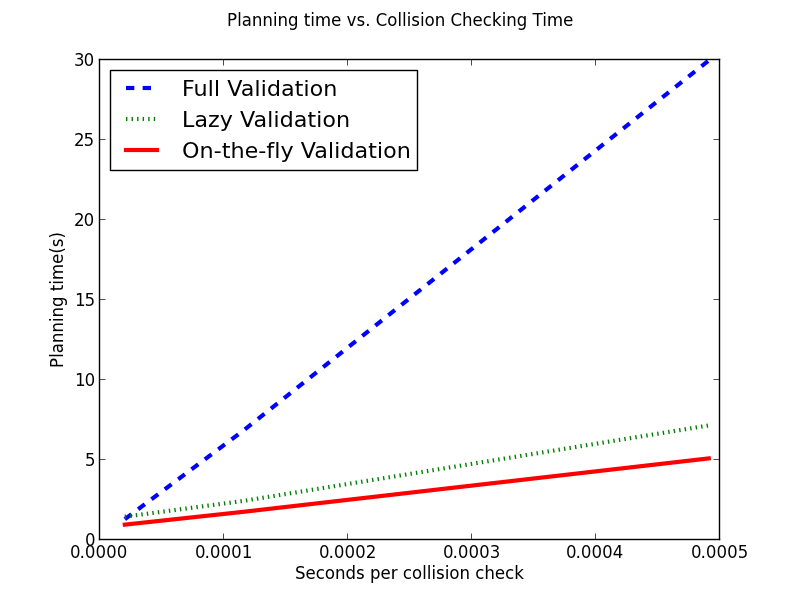
\includegraphics[width=1\columnwidth]{full_lazy_onthefly2.png}
%    \caption{A comparison between the lazy validation and full validation method
%    over different speeds of collision checking. These results were generated by
%artificially slowing the SBPL collision checker performance to various speeds. }
%    \figlab{egraph_size_cc}
%\end{figure}


\begin{table}[t]
    \begin{center}
        \begin{tabular}{| l | l | l | l | l | }
            \hline
            & Lazy & Full & On-the-fly & RRTConnect \\ \hline
            Average Path Quality & 1.60 & 1.69 & 1.72 & 2.15 \\ \hline
        \end{tabular}
    \end{center}
    \caption{Path quality comparison between three E-Graph methods and
    RRTConnect. All E-Graph methods are initialized with an E-Graph of 7000
vertices.}
    \tablab{pquality}
\end{table}

In terms of path quality, all three E-Graph methods are nearly identical, as
seen in \tabref{pquality}.

\section{Conclusion}
In this work, we have presented a method for leveraging a large amount of prior
experiences to accelerate planning in scenarios with random clutter. We augment
the existing E-Graph planning framework to lazily validate experiences in the
E-Graph, which allowed our method to only expend computation on validating portions
of prior experience that are relevant to the particular planning episode. We
show experimental results that demonstrate the speedup in a mailroom environment
compared to a number of other possible methods.

In future work, we will explore obstacle modeling methods to decrease the number
of overall replans required when many obstacles are added to the environment. In
addition, we will look into possible offline computations to improve
the accuracy of edge invalidations along with pruning or improving the quality
of the E-Graph when there is spare time.

\section{Acknowledgements}
We thank Google for their support of these efforts. This research was also sponsored by ONR grant N00014-09-1-1052.
We also thank Ben Cohen for his invaluable input.

\bibliographystyle{plain}
\bibliography{references}
\end{document}
